\tikzstyle{place}=[circle, draw, fill=black, inner sep=0pt, thick, minimum size=2mm]
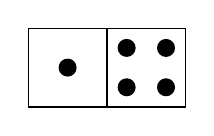
\begin{tikzpicture}
   \def\rectanglepath{-- ++(1cm,0cm)-- ++(0cm,1cm)-- ++(-1cm,0cm) -- cycle}
   \draw (0,0) \rectanglepath;
   \draw (1,0) \rectanglepath;
   \node [place] at (0.5,0.5)   {};
   \node [place] at (1.25,0.75) {};
   \node [place] at (1.25,0.25) {};
   \node [place] at (1.75,0.75) {};
   \node [place] at (1.75,0.25) {};
\end{tikzpicture}
